\chapter{Биттік манипуляциялау}

Компьютер бағдарламаларындағы барлық деректер 
биттер арқылы, яғни 0 және 1 сандарымен сақталған.
Бұл тарауда бүтін сандардың биттік көрсетілімі мен 
биттік операциялар қолданысының үлгілерін талқылаймыз.
Алгоритмдік бағдарламалауда биттік манипуляциялаудың көп жағдайда
пайдалы екендігі байқалады. 
% It turns out that there are many uses for
% bit manipulation in algorithm programming.

\section{Биттік көрсетілім}

\index{биттік көрсетілім}

Бағдарламалауда $n$ биттік саны $n$ биттен тұратын бинарлы сан ретінде сақталады.
Мысалы, C++ \texttt{int} типі -- 32 биттік, 
бұл әр \texttt{int} саны 32 биттен тұратындығын білдіреді.

Төменде 43 \texttt{int} санының биттік көрсетілімі берілген:
\[00000000000000000000000000101011\]
Көрсетілімдегі биттер оңнан солға қарай индекстелген.
$b_k \cdots b_2 b_1 b_0$ биттік көрсетілімін 
санға айналдыру үшін \[b_k 2^k + \ldots + b_2 2^2 + b_1 2^1 + b_0 2^0\] формуласын қолдана аламыз. 
Мысалы:
\[1 \cdot 2^5 + 1 \cdot 2^3 + 1 \cdot 2^1 + 1 \cdot 2^0 = 43.\]

Санның биттік көрсетілімі таңбалы немесе таңбасыз болып бөлінеді.
Әдетте біз таңбалы көрсетілімді қолданамыз. Оның көмегімен
оң және теріс  таңбалы сандардың екі түрі де көрсетіле береді.
Таңбалы $n$ битті айнымалы кез келген $-2^{n-1}$ және $2^{n-1}-1$
аралығындағы бүтін санды қамтиды. Мысалы, С++-тегі \texttt{int} типі --
таңбалы тип, сондықтан \texttt{int} айнымалысы $-2^{31}$ және $2^{31}-1$
аралығындағы кез келген бүтін санды қамти алады.

Таңбалы көрсетілімдегі бірінші бит -- санның таңбасы
(оң сандар үшін 0, теріс сандар үшін 1),  
ал қалған $n-1$ бит -- санның мөлшері.
\key{Қосымша кодтау} деп сандағы 
биттердің барлығын кері аударып, кейін бірге арттыру
арқылы қарама-қарсы санды табу операциясын айтамыз. % todo: қосымша код is noun, but here I think it's defined as verb

$-43$ \texttt{int} санының   
биттік көрсетілімін мысал ретінде келтірейік: 
\[11111111111111111111111111010101.\]

Таңбасыз көрсетілімде тек қана оң сандар қолданыла алады,
бірақ сандар мәнінің жоғарғы шегі биік болады.
Таңбасыз $n$ битті айнымалы $0$ мен $2^n-1$ 
аралығындағы кез келген бүтін санды қамти алады.
Мысалы, С++-те \texttt{unsigned int} айнымалысы кез келген 
$0$ мен $2^{32}-1$ аралығындағы бүтін санды қамти алады.

Көрсетілімдер арасындағы байланыс:
таңбалы $-x$ саны таңбасыз $2^n-x$ санына тең.
Мысалы, төмендегі код таңбалы $x=-43$ санының 
таңбасыз $y=2^{32}-43$ санына тең екендігін көрсетеді:
\begin{lstlisting}
int x = -43;
unsigned int y = x;
cout << x << "\n"; // -43
cout << y << "\n"; // 4294967253
\end{lstlisting}

Егер сан биттік көрсетілімнің жоғарғы шегінен асса,
санның асатолуы орын алады. 
Таңбалы көрсетілімде $2^{n-1}-1$-ден кейінгі сан -- $-2^{n-1}$,
ал таңбасыз көрсетілімде $2^n-1$-ден кейінгі сан -- $0$.
Мысалға келесі кодты қарастырайық:
\begin{lstlisting}
int x = 2147483647
cout << x << "\n"; // 2147483647
x++;
cout << x << "\n"; // -2147483648
\end{lstlisting}

Бастапқыда $x$-тің мәні $2^{31}-1$-ге тең.
Бұл -- \texttt{int} айнымалысында сақтала 
алатын ең үлкен мән, сондықтан $2^{31}-1$-ден
кейінгі мән -- $-2^{31}$ болады.

\section{Биттік операциялар}

\newcommand\XOR{\mathbin{\char`\^}}

\subsubsection{Конъюнкция (Биттік және)} 

\index{конъюнкция}

$x$ \& $y$ \key{конъюнкциясы} (биттік жәнесі) $x$ пен $y$ -тің екеуі де бір бит болатын
позициялардағы жазылуы бір биттік санды шығарады.
% The \key{and} operation $x$ \& $y$ produces a number
% that has one bits in positions where both
% $x$ and $y$ have one bits.
Мысалы, $22$ \& $26$ = 18, себебі

\begin{center}
\begin{tabular}{rrr}
& 10110 & (22)\\
\& & 11010 & (26) \\
\hline
 = & 10010 & (18) \\
\end{tabular}
\end{center}

Конъюнкцияны қолдану арқылы $x$ санының жұп немесе тақ екенін тексере аламыз. Егер $x$ жұп болса, $x$ \& $1$ = 0-ге, ал
егер $x$ тақ болса, $x$ \& $1$ = 1-ге тең.

Қорыта айтқанда, $x$ \& $(2^k-1)$ = 0
болғанда ғана $x$ $2^k$-ге  бөлінеді.

\subsubsection{Дизъюнкция (Биттік немесе)} 

\index{дизъюнкция}

$x$ | $y$ \key{дизъюнкциясы} (биттік немесесі) $x$ пен $y$ кем дегенде 
екеуінің бірінде бит болатын
позицияларда бір бит жазылған санды құрайды. 
Мысалы, $22$ | $26$ = 30, себебі

\begin{center}
\begin{tabular}{rrr}
& 10110 & (22)\\
| & 11010 & (26) \\
\hline
 = & 11110 & (30) \\
\end{tabular}
\end{center}

\subsubsection{Жоюшы дизъюнкция (xor)} %жоюшы немесе 

\index{жоюшы дизъюнкция}

$x$ $\XOR$ $y$ \key{жоюшы дизъюнкциясы} (xor) екеуінің 
бірінде ғана бір бит болатын
позицияларда бір бит жазылған санды құрайды.
Мысалы, $22$ $\XOR$ $26$ = 12, себебі 

\begin{center}
\begin{tabular}{rrr}
& 10110 & (22)\\
$\XOR$ & 11010 & (26) \\
\hline
 = & 01100 & (12) \\
\end{tabular}
\end{center}

\subsubsection{Биттік терістеу} 

\index{биттік терістеу}

\textasciitilde$x$ \key{биттік терістеуі}
$x$-тің барлық биттері кері аударылатын санды құрайды. Бұл жағдайда
\textasciitilde$x = -x-1$ формуласы қолданылады, мысалы,
\textasciitilde$29 = -30$.

Биттік терістеудің бит деңгейіндегі нәтижесі 
көрсетілімнің ұзындығына байланысты болып келеді.
Себебі операция барлық биттерді кері аударады.
Мысалы, егер сандар 32-биттік \texttt{int} болса, 
төмендегі нәтиже алынады:

\begin{center}
\begin{tabular}{rrrr}
$x$ & = & 29 &   00000000000000000000000000011101 \\
\textasciitilde$x$ & = & $-30$ & 11111111111111111111111111100010 \\
\end{tabular}
\end{center}

\subsubsection{Биттік ығысулар}

\index{биттік ығысу}

Сол жақ биттік ығысу $x < < k$ санға $k$
нөл биттерін қосады, ал оң жақ биттік ығысу 
$x > > k$ саннан соңғы $k$ нөл биттерін өшіреді.
Мысалы, $14 < < 2 = 56$, себебі $14$ пен $56$ 1110 және 111000
биттік көрсетілімдерімен сәйкес келеді. Сол сияқты $49 > > 3 = 6$,
себебі $49$ пен $6$ 110001 және 110 биттік көрсетілімдеріне сәйкес келеді.

$x < < k$ $x$-ті $2^k$ көбейтіп, $x > > k$ $x$-ті
$2^k$ бөліп, төменге бүтін санға дейін 
дөңгелектейтінін ескеріңіз.

\subsubsection{Қолданылулар}

$1 < < k$ формасындағы санның $k$-позициясында 1 бит, ал қалған 
позицияларында 0 бит болады, мұндай сандарды сандағы жекелеген 
биттерге қол жеткізу үшін қолдана аламыз.
Көбіне $x$ \& $(1 < < k)$ нөл болмаған жағдайда ғана санның $k$-биті бір болады.
Келесі код \texttt{int} $x$ санының биттік көрсетілімін шығарады:

\begin{lstlisting}
for (int i = 31; i >= 0; i--) {
    if (x&(1<<i)) cout << "1";
    else cout << "0";
}
\end{lstlisting}

Санның жекелеген биттерін ұқсас идеяларды қолдану арқылы
анықтауға болады. Мысалы, $x$ | $(1 < < k)$ формуласы $x$-тің 
$k$-битін бір деп белгілейді, $x$ \& \textasciitilde $(1 < < k)$
формуласы $x$-тің $k$-битін нөл деп белгілейді, ал $x$ $\XOR$ $(1 < < k)$
формуласы $x$-тің $k$-битін терістейді.

$x$ \& $(x-1)$ формуласы $x$-тің соңғы бір битін нөл деп белгілейді,
ал $x$ \& $-x$ формуласы соңғысынан басқа барлық бір биттерін нөл 
деп белгілейді. $x$ | $(x-1)$ формуласы соңғы бір битінен кейінгі
барлық биттерді терістейді. Сонымен қатар оң $x$ саны $x$ \& $(x-1) = 0$
болған жағдайда екінің дәрежесі болатынын ескерген жөн.

\subsubsection*{Қосымша функциялар}

g++ компиляторы биттерді санау үшін келесі 
функциялармен қамтамасыз етеді:

% The g++ compiler provides the following
% functions for counting bits:

\begin{itemize}
\item
$\texttt{\_\_builtin\_clz}(x)$:
санның басындағы нөлдер саны
% the number of zeros at the beginning of the number
\item
$\texttt{\_\_builtin\_ctz}(x)$:
санның соңындағы нөлдер саны
% the number of zeros at the end of the number
\item
$\texttt{\_\_builtin\_popcount}(x)$:
сандағы бірлер саны
% the number of ones in the number
\item
$\texttt{\_\_builtin\_parity}(x)$:
сандағы бірлер санының жұптығы (тақ немесе жұп)
% the parity (even or odd) of the number of ones
\end{itemize}
\begin{samepage}

Функциялар төмендегідей жолмен қолданылады:
\begin{lstlisting}
int x = 5328; // 00000000000000000001010011010000
cout << __builtin_clz(x) << "\n"; // 19
cout << __builtin_ctz(x) << "\n"; // 4
cout << __builtin_popcount(x) << "\n"; // 5
cout << __builtin_parity(x) << "\n"; // 1
\end{lstlisting}
\end{samepage}

Жоғарыдағы функциялар \texttt{int} типіндегі сандарды ғана қолдайды. 
\texttt{long long} типіндегі сандармен жұмыс жасау үшін функциялардың
атауларына \texttt{ll} суффиксін қосу керек. 

% While the above functions only support \texttt{int} numbers,
% there are also \texttt{long long} versions of
% the functions available with the suffix \texttt{ll}.

\section{Жиындар көрсетілімі}

$\{0,1,2,\ldots,n-1\}$ жиынының әр ішжиыны 
$n$ биттік бүтін сан ретінде көрсетіле алады,
ондағы әр бірлік қай элемент жиынға жататынын 
анықтайды. Бұл -- жиынды көрсетудің тиімді жолы,
себебі әр элемент тек бір бит жадыны талап етеді
және жиын операциялары бит операциялары сияқты
орындала алады.

Мысалы, \texttt{int} 32-биттік тип болғандықтан 
\texttt{int} саны $\{0,1,2,\ldots,31\}$ жиынының кез келген 
ішжиынын көрсете алады. $\{1,3,4,8\}$ жиынының биттік көрсетілімі 
$2^8+2^4+2^3+2^1=282$ санына сәйкес төмендегідей болады: 
\[00000000000000000000000100011010.\]

\subsubsection{Жиын орындалуы}

Келесі код $\{0,1,2,\ldots,31\}$ ішжиынын қамти алатын
\texttt{int} $x$ айнымалысын жариялайды.
Бұдан соң код 1, 3, 4 және 8 элементтерін
жиынға қосып, жиынның өлшемін шығарады:
\begin{lstlisting}
int x = 0;
x |= (1<<1);
x |= (1<<3);
x |= (1<<4);
x |= (1<<8);
cout << __builtin_popcount(x) << "\n"; // 4
\end{lstlisting}
Ал келесі код жиынға жататын барлық 
элементтерді шығарады:
\begin{lstlisting}
for (int i = 0; i < 32; i++) {
    if (x&(1<<i)) cout << i << " ";
}
// output: 1 3 4 8 
\end{lstlisting}

\subsubsection{Жиын операциялары}

Жиын операциялары бит операциялары сияқты төмендегі түрде орындалады:

\begin{center}
\begin{tabular}{lll}
& жиын синтаксы & бит синтаксы \\
\hline
қиылысу & $a \cap b$ & $a$ \& $b$ \\
бірігу & $a \cup b$ & $a$ | $b$ \\
толықтыру & $\bar a$ & \textasciitilde$a$ \\
айырма & $a \setminus b$ & $a$ \& (\textasciitilde$b$) \\
\end{tabular}
\end{center}

Мысалы, келесі код алдымен $x=\{1,3,4,8\}$ және $y=\{3,6,8,9\}$
жиындарын құрайды, содан кейін ғана $z = x \cup y = \{1,3,4,6,8,9\}$
жиынын құрайды:

\begin{lstlisting}
int x = (1<<1)|(1<<3)|(1<<4)|(1<<8);
int y = (1<<3)|(1<<6)|(1<<8)|(1<<9);
int z = x|y;
cout << __builtin_popcount(z) << "\n"; // 6
\end{lstlisting}

\subsubsection{Ішжиынды өтіп шығу}

Келесі код $\{0,1,\ldots,n-1\}$ ішжиындарын 
өтіп шығады:

\begin{lstlisting}
for (int b = 0; b < (1<<n); b++) {
    // process subset b
}
\end{lstlisting}
Төмендегі код дәл $k$ элементі бар ішжиындарды
өтіп шығады:
\begin{lstlisting}
for (int b = 0; b < (1<<n); b++) {
    if (__builtin_popcount(b) == k) {
        // process subset b
    }
}
\end{lstlisting}
Келесі код $x$ жиынының ішжиындарын өтіп шығады:
\begin{lstlisting}
int b = 0;
do {
    // process subset b
} while (b=(b-x)&x);
\end{lstlisting}

\section{Бит оңтайландырулары}

Көптеген алгоритмдер бит операцияларын
қолдану арқылы оңтайландырыла алады. 
Мұндай оңтайландырулар алгоритмнің
уақытша күрделілігін өзгертпейді,
бірақ олар кодтың нақты орындалу
уақытына үлкен әсерін тигізе алады.
% Such optimizations do not change the
% time complexity of the algorithm,
% but they may have a large impact
% on the actual running time of the code.
Бұл бөлікте осындай мысалдарды қарастырамыз.

\subsubsection{Хемминг арақашықтығы}

\index{Хемминг арақашықтығы}

$\texttt{hamming}(a,b)$ \key{Хемминг арақашықтығы} --
ұзындықтары бірдей $a$ және $b$ жолдарының өзгешеленетін 
позициялар саны.
Мысалы,
\[\texttt{hamming}(01101,11001)=2.\]

Келесі есепті қарастырайық:
$n$ бит жолдарының тізімі берілген, әрқайсының ұзындығы $k$,
тізімдегі екі жол арасындағы минималды Хемминг арақашықтығын 
есептеңіз.
Мысалы, $[00111,01101,11110]$ жауабы -- 2, себебі 
\begin{itemize}[noitemsep]
\item $\texttt{hamming}(00111,01101)=2$,
\item $\texttt{hamming}(00111,11110)=3$, және
\item $\texttt{hamming}(01101,11110)=3$.
\end{itemize}

Есепті шығарудың оңай жолы -- барлық жолдардың жұптарын қарастырып,
олардың Хемминг арақашықтықтарын есептеу, бұл $O(n^2 k)$ уақыт алады.
Арақашықтықты есептеу үшін келесі функцияны қолдануға болады:
\begin{lstlisting}
int hamming(string a, string b) {
    int d = 0;
    for (int i = 0; i < k; i++) {
        if (a[i] != b[i]) d++;
    }
    return d;
}
\end{lstlisting}

Егер $k$ кіші болса, біз кодты бит жолдарын 
бүтін сандар ретінде сақтап, Хемминг арақашықтықтарын 
бит операцияларын қолданып шығару арқылы оңтайландыра аламыз.
Егер $k \le 32$ болса, көбіне жолдарды жай ғана \texttt{int} мәндері 
ретінде сақтап, келесі функциямен арақашықтықты есептей береміз:
\begin{lstlisting}
int hamming(int a, int b) {
    return __builtin_popcount(a^b);
}
\end{lstlisting}
Жоғарыдағы функцияда жоюшы дизъюнкция (xor) $a$ мен $b$
жолдары өзгешеленетін позицияларда бір бит болатындай
биттік жол құрайды. Кейін биттер саны 
\texttt{\_\_builtin\_popcount} функциясы арқылы есептеледі.

Орындалуларды салыстыру үшін біз ұзындығы 30
болатын 1000 кездейсоқ бит жолдарының тізімін құрдық. Бірінші тәсілді қолданғандағы
ізденіс 13.5 секунд алса, бит оңтайландыруынан кейін ол бар болғаны 0.5 секундта орындалды. Осылайша биттік оңтайландырылған код бастапқы кодтан
шамамен 30 есе тезірек жұмыс істейді.

\subsubsection{Ішкі торларды есептеу}

Басқа мысал ретінде келесі есепті қарастырайық:
$n \times n$ тор берілген, әр ұяшығы қара (1) немесе
ақ (0), барлық бұрыштары қара болатын ішкі торлар санын
есептеңіз.
Мысалы, мына тор
\begin{center}
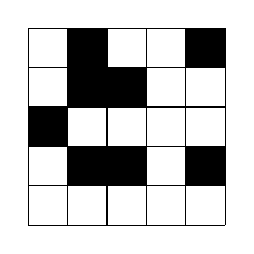
\begin{tikzpicture}[scale=0.5]
\fill[black] (1,1) rectangle (2,2);
\fill[black] (1,4) rectangle (2,5);
\fill[black] (4,1) rectangle (5,2);
\fill[black] (4,4) rectangle (5,5);
\fill[black] (1,3) rectangle (2,4);
\fill[black] (2,3) rectangle (3,4);
\fill[black] (2,1) rectangle (3,2);
\fill[black] (0,2) rectangle (1,3);
\draw (0,0) grid (5,5);
\end{tikzpicture}
\end{center}
сондай екі ішкі тор қамтиды:
\begin{center}
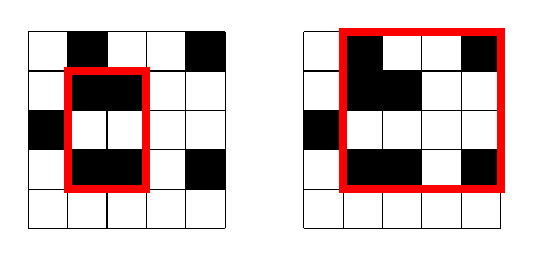
\begin{tikzpicture}[scale=0.5]
\fill[black] (1,1) rectangle (2,2);
\fill[black] (1,4) rectangle (2,5);
\fill[black] (4,1) rectangle (5,2);
\fill[black] (4,4) rectangle (5,5);
\fill[black] (1,3) rectangle (2,4);
\fill[black] (2,3) rectangle (3,4);
\fill[black] (2,1) rectangle (3,2);
\fill[black] (0,2) rectangle (1,3);
\draw (0,0) grid (5,5);

\fill[black] (7+1,1) rectangle (7+2,2);
\fill[black] (7+1,4) rectangle (7+2,5);
\fill[black] (7+4,1) rectangle (7+5,2);
\fill[black] (7+4,4) rectangle (7+5,5);
\fill[black] (7+1,3) rectangle (7+2,4);
\fill[black] (7+2,3) rectangle (7+3,4);
\fill[black] (7+2,1) rectangle (7+3,2);
\fill[black] (7+0,2) rectangle (7+1,3);
\draw (7+0,0) grid (7+5,5);

\draw[color=red,line width=1mm] (1,1) rectangle (3,4);
\draw[color=red,line width=1mm] (7+1,1) rectangle (7+5,5);
\end{tikzpicture}
\end{center}

Есепті $O(n^3)$ уақытында келесі алгоритммен шығаруға болады. Барлық $O(n^2)$ қатарлар жұптарын өтіп шығып,
әр $(a,b)$ жұбы үшін екі қатарда да қара 
ұяшық болатындай бағандар санын $O(n)$ 
уақытта есептейміз. Келесі код $\texttt{color}[y][x]$ --
$y$ қатары мен $x$ бағанындағы түсті білдіреді деп қарастырады:
\begin{lstlisting}
int count = 0;
for (int i = 0; i < n; i++) {
    if (color[a][i] == 1 && color[b][i] == 1) count++;
}
\end{lstlisting}
Кейін бұл бағандардан $\texttt{count}(\texttt{count}-1)/2$ 
бұрыштары қара ішкі торлар санын есептейміз. Себебі кез келген
екеуін таңдап, ішкі тор құруға болады.

Аталған алгоритмді оңтайландыру үшін торды бағандар блоктарына бөлеміз,
блоктардың әрқайсысы $N$ қатарлас келген бағаналардан тұрады. Кейін әр қатар $N$-биттік сандар тізімі ретінде сақталады, әр бит ұяшықтың түсін білдіреді.
Енді $N$ бағанды бір сәтте бит операцияларын қолдана отырып, 
өңдей аламыз. Келесі кодтағы $\texttt{color}[y][k]$
$N$ түстерден тұратын блокты биттер түрінде ұсынады.
% In the following code, $\texttt{color}[y][k]$ represents
% a block of $N$ colors as bits.
\begin{lstlisting}
int count = 0;
for (int i = 0; i <= n/N; i++) {
    count += __builtin_popcount(color[a][i]&color[b][i]);
}
\end{lstlisting}
Нәтижесінде пайда болған алгоритм $O(n^3/N)$ уақытта 
жұмыс істейді.

$2500 \times 2500$ өлшемді кездейсоқ тор құрастырып, 
бастапқы және биттік оңтайландырудан кейінгі орындалуларды 
салыстырдық. Бастапқы код $29.6$ секундта орындалса, 
биттік оңтайландырудан кейінгі орындалу $N=32$ (\texttt{int} сандарымен)
$3.1$ секундты, ал $N=64$ (\texttt{long long} сандарымен) $1.7$ секундты 
қажет етті.

\section{Динамикалық бағдарламалау}

Биттік операциялар күйлері элементтер ішжиындарын қамтитын 
динамикалық бағдарламалау алгоритмдерінің
тиімді және қолайлы орындалуына септігін тигізеді,
себебі мұндай күйлер бүтін сандар ретінде сақтала алады.
Келесі қарастыратын мысалдарда биттік операциялар мен 
динамикалық бағдарламалау өзара біріктірілген.

\subsubsection{Оңтайлы іріктеу}

Алғашқы мысал ретінде келесі есепті қарастыруға болады. 
Бізге $n$ күндегі $k$ тауарлардың бағалары берілген, әр тауарды бірден сатып алғымыз келеді. Бірақ әр күні бір ғана тауар
сатып ала аламыз. Минималды жалпы құн қанша екенін анықтауымыз керек. Үлгі ретінде келесі
жағдайды қарастырайық ($k=3$ және $n=8$):
\begin{center}
\begin{tikzpicture}[scale=.65]
    \draw (0, 0) grid (8,3);
    \node at (-2.5,2.5) {тауар 0};
    \node at (-2.5,1.5) {тауар 1};
    \node at (-2.5,0.5) {тауар 2};

    \foreach \x in {0,...,7}
        {\node at (\x+0.5,3.5) {\x};}
    \foreach \x/\v in {0/6,1/9,2/5,3/2,4/8,5/9,6/1,7/6}
        {\node at (\x+0.5,2.5) {\v};}
    \foreach \x/\v in {0/8,1/2,2/6,3/2,4/7,5/5,6/7,7/2}
        {\node at (\x+0.5,1.5) {\v};}
    \foreach \x/\v in {0/5,1/3,2/9,3/7,4/3,5/5,6/1,7/4}
        {\node at (\x+0.5,0.5) {\v};}
\end{tikzpicture}
\end{center}
Бұл жағдайдағы минималды жалпы құн -- $5$:
\begin{center}
\begin{tikzpicture}[scale=.65]
    \fill [color=lightgray] (1, 1) rectangle (2, 2);
    \fill [color=lightgray] (3, 2) rectangle (4, 3);
    \fill [color=lightgray] (6, 0) rectangle (7, 1);
    \draw (0, 0) grid (8,3);
    \node at (-2.5,2.5) {тауар 0};
    \node at (-2.5,1.5) {тауар 1};
    \node at (-2.5,0.5) {тауар 2};

    \foreach \x in {0,...,7}
        {\node at (\x+0.5,3.5) {\x};}
    \foreach \x/\v in {0/6,1/9,2/5,3/2,4/8,5/9,6/1,7/6}
        {\node at (\x+0.5,2.5) {\v};}
    \foreach \x/\v in {0/8,1/2,2/6,3/2,4/7,5/5,6/7,7/2}
        {\node at (\x+0.5,1.5) {\v};}
    \foreach \x/\v in {0/5,1/3,2/9,3/7,4/3,5/5,6/1,7/4}
        {\node at (\x+0.5,0.5) {\v};}
\end{tikzpicture}
\end{center}

$\texttt{price}[x][d]$ $x$ тауарының $d$ күніндегі бағасы деп белгілейік.
Мысалы, жоғарыдағы жағдайда $\texttt{price}[2][3] = 7$.
$\texttt{total}(S,d)$ $S$ тауарлар ішжиынын $d$ күні сатып алғандағы 
минималды жалпы құн деп белгілейік. Бұл функцияны қолдану арқылы есеп шешімі 
$\texttt{total}(\{0 \ldots k-1\},n-1)$ болмақ.

Алғашында $\texttt{total}(\emptyset,d) = 0$, себебі 
бос жиынды сатып алу бағасы жоқ, онымен қоса 
$\texttt{total}(\{x\},0) = \texttt{price}[x][0]$.
Себебі бірінші күні тауарды сатып алудың жалғыз жолы бар.
Кейін төмендегі рекурсияны қолдана аламыз:
\begin{equation*}
\begin{split}
\texttt{total}(S,d) = \min( & \texttt{total}(S,d-1), \\
& \min_{x \in S} (\texttt{total}(S \setminus x,d-1)+\texttt{price}[x][d]))
\end{split}
\end{equation*}
Бұл $d$ күні $S$-ке жататын қандай да бір $x$ тауарын сатып алатынымызды не сатып алмайтынымызды білдіреді. Екінші жағдайда $x$-ті $S$-тен өшіріп, $x$ бағасын 
жалпы құнға қосамыз.

Келесі қадам -- динамикалық бағдарламалау көмегімен функция мәндерін есептеу.
Функция мәндерін сақтау үшін келесі жиымды құрастырамыз: 
\begin{lstlisting}
int total[1<<K][N];
\end{lstlisting}
Мұндағы $K$ мен $N$ жарамды көлемде алынған, ал жиымдағы бірінші шама -- ішжиынның биттік көрсетілімі.

Алдымен $d=0$ болған жағдайларды өңдейміз:
\begin{lstlisting}
for (int x = 0; x < k; x++) {
    total[1<<x][0] = price[x][0];
}
\end{lstlisting}
Кейін рекурсия төмендегідей кодқа ауысады:
\begin{lstlisting}
for (int d = 1; d < n; d++) {
    for (int s = 0; s < (1<<k); s++) {
        total[s][d] = total[s][d-1];
        for (int x = 0; x < k; x++) {
            if (s&(1<<x)) {
                total[s][d] = min(total[s][d],
                                    total[s^(1<<x)][d-1]+price[x][d]);
            }
        }
    }
}
\end{lstlisting}
Алгоритмнің уақытша күрделілігі -- $O(n 2^k k)$.

\subsubsection{Алмастырулардан ішжиындарға} % From permutations to subsets

Динамикалық бағдарламалауды қолданып, алмастырулар итерациясын
ішжиындар итерациясына алмастыра аламыз\footnote{Бұл
тәсілді 1962 жылы М.Хелд пен Р.М.Карп таныстырды\cite{hel62}.}.
Мұндағы артықшылық алмастырулар саны -- $n!$ ішжиындар саны -- $2^n$-нен
анағұрлым үлкен болуында жатыр. Мысалы, егер $n=20$ болса, 
$n! \approx 2.4 \cdot 10^{18}$, ал $2^n \approx 10^6$.
Сондықтан кейбір $n$ мәндері үшін алмастырулар емес, ішжиындарды
өтіп шығу тиімдірек болмақ.

Мысал ретінде келесі есепті қарастырайық:
Максималды жүк салмағы $x$ болатын лифт пен 
салмақтары белгілі $n$ адам бар. Олар төменгі
қабаттан жоғарғы қабатқа көтерілгісі келеді.
Егер адамдардың міну ретін оңтайландырса,
ең азы қанша сапар жасалуы қажет?

Мысалы, $x=10$, $n=5$ деп алайық. Ал
салмақтары төмендегідей болсын: 
\begin{center}
\begin{tabular}{ll}
адам & салмақ \\
\hline
0 & 2 \\
1 & 3 \\
2 & 3 \\
3 & 5 \\
4 & 6 \\
\end{tabular}
\end{center}
Бұл жағдайда минималды сапарлар саны -- 2.
Оңтайлы реттілік -- $\{0,2,3,1,4\}$, ол
адамдарды екі сапарға бөледі: бірінші $\{0,2,3\}$ (жалпы салмағы 10),
ал кейін $\{1,4\}$ (жалпы салмағы 9).

Есеп $O(n! n)$ уақыт ішінде барлық мүмкін болатын $n$ адам
алмастыруларын тексеру арқылы $O(n! n)$ уақытында оңай шешіледі.
Бірақ $O(2^n n)$ уақытында орындалатын тиімдірек динамикалық бағдарламалау алгоритмін
қолдана аламыз. Идеясы -- әр адамдар ішжиыны үшін екі мәнді, атап айтқанда қажетті минималды сапар саны 
мен соңғы сапардағы адамдар тобының минималды салмағын сақтаймыз. 

$\texttt{weight}[p]$ $p$ адамның салмағын белгілейді десек, екі функцияны көрсетеміз. Олар: 
$\texttt{rides}(S)$ -- $S$ ішжиыны үшін минималды сапар саны,
$\texttt{last}(S)$ -- соңғы сапардағы минималды салмақ.
Мысалы, жоғарыдағы жағдайда 
\[ \texttt{rides}(\{1,3,4\})=2 \hspace{10px} \textrm{және}
\hspace{10px} \texttt{last}(\{1,3,4\})=5,\]
себебі оңтайлы сапарлар -- $\{1,4\}$ және $\{3\}$,
сонымен қоса екінші сапардың салмағы -- 5. 
Әрине, біздің ақырғы нысанымыз $\texttt{rides}(\{0 \ldots n-1\})$ 
мәнін есептеу.

Функциялардың мәндерін рекурсивті 
түрде есептеп, кейін динамикалық
бағдарламалауды қолдануымызға болады.
Мұндағы идея $S$-ке тиесілі барлық адамдарды
өтіп шығып, лифтке ең соңғы болып кіретін $p$ адамды
оңтайлы таңдауға негізделеді. Әрбір осындай таңдау адамдардың ішжиынына арналған ішесептерге әкеледі.
Егер $\texttt{last}(S \setminus p)+\texttt{weight}[p] \le x$ болса,
біз $p$-ді соңғы сапарға қосамыз. Әйтпесе бастапқыда тек қана $p$ болатын жаңа сапарды кейінге сақтауға тура келеді.

% We can calculate the values
% of the functions recursively and then apply
% dynamic programming.
% The idea is to go through all people
% who belong to $S$ and optimally
% choose the last person $p$ who enters the elevator.
% Each such choice yields a subproblem
% for a smaller subset of people.
% If $\texttt{last}(S \setminus p)+\texttt{weight}[p] \le x$,
% we can add $p$ to the last ride.
% Otherwise, we have to reserve a new ride
% that initially only contains $p$.

Динамикалық бағдарламалауды орындау мақсатында
әр $S$ ішжиыны үшін
$(\texttt{rides}(S),\texttt{last}(S))$ жұбын сақтайтын келесі жиымды жариялаймыз:
\begin{lstlisting}
pair<int,int> best[1<<N];
\end{lstlisting}
Бос топтың мәнін төмендегідей үлгіде меншіктейміз:
\begin{lstlisting}
best[0] = {1,0};
\end{lstlisting}
Кейін жиымды келесідей тәртіппен толтырамыз:

% To implement dynamic programming,
% we declare an array
% \begin{lstlisting}
% pair<int,int> best[1<<N];
% \end{lstlisting}
% that contains for each subset $S$
% a pair $(\texttt{rides}(S),\texttt{last}(S))$.
% We set the value for an empty group as follows:
% \begin{lstlisting}
% best[0] = {1,0};
% \end{lstlisting}
% Then, we can fill the array as follows:

\begin{lstlisting}
for (int s = 1; s < (1<<n); s++) {
    // initial value: n+1 rides are needed
    best[s] = {n+1,0};
    for (int p = 0; p < n; p++) {
        if (s&(1<<p)) {
            auto option = best[s^(1<<p)];
            if (option.second+weight[p] <= x) {
                // add p to an existing ride
                option.second += weight[p];
            } else {
                // reserve a new ride for p
                option.first++;
                option.second = weight[p];
            }
            best[s] = min(best[s], option);
        }
    }
}
\end{lstlisting}
Жоғарыда келтірілген циклдің $S_1 \subset S_2$ болатын
кез келген $S_1$ және $S_2$
ішжиындары үшін $S_1$ $S_2$-ден бірінші өңделетініне кепілдік беретініне назар аударғанымыз жөн.
Осылайша динамикалық бағдарламалау мәндері дұрыс ретпен есептеледі.
% Note that the above loop guarantees that
% for any two subsets $S_1$ and $S_2$
% such that $S_1 \subset S_2$, we process $S_1$ before $S_2$.
% Thus, the dynamic programming values are calculated in the
% correct order.

\subsubsection{Ішжиындар мәндерінің қосындысы} %Counting subsets

Бөлімнің соңғы есебіне келейік. 
$X=\{0 \ldots n-1\}$ жиыны мен әр $S \subset X$
ішжиынына сәйкес $\texttt{value}[S]$ бүтін мәні берілген.
Әр $S$-ке
\[\texttt{sum}(S) = \sum_{A \subset S} \texttt{value}[A],\]
қосындысын есептеу, яғни $S$ ішжиындарының мәндер қосындысын есептеу тапсырма ретінде беріліп тұр.

% Our last problem in this chapter is as follows:
% Let $X=\{0 \ldots n-1\}$, and each subset $S \subset X$
% is assigned an integer $\texttt{value}[S]$.
% Our task is to calculate for each $S$
% \[\texttt{sum}(S) = \sum_{A \subset S} \texttt{value}[A],\]
% i.e., the sum of values of subsets of $S$.

Мысалы, $n=3$ деп есептейік және келесі мәндер берілген делік:
% For example, suppose that $n=3$ and the values are as follows:
\begin{multicols}{2}
\begin{itemize}
\item $\texttt{value}[\emptyset] = 3$
\item $\texttt{value}[\{0\}] = 1$
\item $\texttt{value}[\{1\}] = 4$
\item $\texttt{value}[\{0,1\}] = 5$
\item $\texttt{value}[\{2\}] = 5$
\item $\texttt{value}[\{0,2\}] = 1$
\item $\texttt{value}[\{1,2\}] = 3$
\item $\texttt{value}[\{0,1,2\}] = 3$
\end{itemize}
\end{multicols}
Ендеше бұл жағдайда:
% In this case, for example,
\begin{equation*}
\begin{split}
\texttt{sum}(\{0,2\}) &= \texttt{value}[\emptyset]+\texttt{value}[\{0\}]+\texttt{value}[\{2\}]+\texttt{value}[\{0,2\}] \\ 
                      &= 3 + 1 + 5 + 1 = 10.
\end{split}
\end{equation*}

Жалпы $2^n$ ішжиын болғандықтан, біз барлық
ішжиындар жұптарынан өту арқылы есепті $O(2^{2n})$ 
уақытта шығара аламыз. Дегенмен динамикалық бағдарламалау
арқылы бұл есепті $O(2^n n)$ уақытта шығаруға болады.
Мұндағы идея $S$-тен өшірілуі мүмкін элементтері шектеулі болатын ішжиымдардың мәндер қосындысына баса назар аударуға бағытталады. % todo: check

% Because there are a total of $2^n$ subsets,
% one possible solution is to go through all
% pairs of subsets in $O(2^{2n})$ time.
% However, using dynamic programming, we
% can solve the problem in $O(2^n n)$ time.
% The idea is to focus on sums where the
% elements that may be removed from $S$ are restricted.

$\texttt{partial}(S,k)$ тек $0 \ldots k$ элементтерін 
өшіруге болатын шектеуі бар $S$ ішжиымдарының
мәндер қосындысы деп белгілейік. 
% Let $\texttt{partial}(S,k)$ denote the sum of
% values of subsets of $S$ with the restriction
% that only elements $0 \ldots k$
% may be removed from $S$.
Мысалы,
\[\texttt{partial}(\{0,2\},1)=\texttt{value}[\{2\}]+\texttt{value}[\{0,2\}],\]
себебі біз тек $0 \ldots 1$ элементтерін өшіре аламыз. 
% because we may only remove elements $0 \ldots 1$.
\texttt{sum} мәндерін \texttt{partial} мәндері арқылы 
есептеуімізге болады, себебі 
% We can calculate values of \texttt{sum} using
% values of \texttt{partial}, because
\[\texttt{sum}(S) = \texttt{partial}(S,n-1).\]
Функцияның негізгі жағдайлары --
% The base cases for the function are
\[\texttt{partial}(S,-1)=\texttt{value}[S],\]
өйткені бұл жағдайда $S$-тен ешқандай элемент өшірілмейді. 
% because in this case no elements can be removed from $S$.
Мұндай жағдайда біз келесі рекуренттік формулаларды қолдана аламыз:
% Then, in the general case we can use the following recurrence:
\begin{equation*}
    \texttt{partial}(S,k) = \begin{cases}
               \texttt{partial}(S,k-1) & k \notin S \\
               \texttt{partial}(S,k-1) + \texttt{partial}(S \setminus \{k\},k-1) & k \in S
           \end{cases}
\end{equation*}
Бұл жерде $k$ элементіне назар аударғанымыз жөн.
Егер $k \in S$ болса, бізде екі таңдау пайда болады. Біз $k$-ны $S$-те
қалдырамыз немесе оны $S$-тен өшіреміз.
% Here we focus on the element $k$.
% If $k \in S$, we have two options: we may either keep $k$ in $S$
% or remove it from $S$.

Қосындыларды есептеп шығаруды жүзеге 
асырудың ерекше ақылды тәсілі бар. Алдымен 
төмендегі жаңа жиымды жариялаймыз.
% There is a particularly clever way to implement the
% calculation of sums. We can declare an array
\begin{lstlisting}
int sum[1<<N];
\end{lstlisting}
% that will contain the sum of each subset.
Бұл жиым әр ішжиынның қосындысын қамтиды.
Жиым төмендегідей түрде инициалданған:
% The array is initialized as follows:
\begin{lstlisting}
for (int s = 0; s < (1<<n); s++) {
    sum[s] = value[s];
}
\end{lstlisting}
Кейін жиымды келісі ретпен толтырамыз:
% Then, we can fill the array as follows:
\begin{lstlisting}
for (int k = 0; k < n; k++) {
    for (int s = 0; s < (1<<n); s++) {
        if (s&(1<<k)) sum[s] += sum[s^(1<<k)];
    }
}
\end{lstlisting}
Бұл код $k=0 \ldots n-1$ үшін $\texttt{partial}(S,k)$ мәндерін 
\texttt{sum} жиымына есептейді. $\texttt{partial}(S,k)$ әрдайым
$\texttt{partial}(S,k-1)$ мәніне негізделгені үшін біз 
\texttt{sum} жиымын қайтадан қолдана аламыз. Ал ол өз кезегінде
ыңғайлы және оңтайлы код жазуға мүмкіндік береді.

% This code calculates the values of $\texttt{partial}(S,k)$
% for $k=0 \ldots n-1$ to the array \texttt{sum}.
% Since $\texttt{partial}(S,k)$ is always based on
% $\texttt{partial}(S,k-1)$, we can reuse the array
% \texttt{sum}, which yields a very efficient implementation.